%% This is an example first chapter.  You should put chapter/appendix that you
%% write into a separate file, and add a line \include{yourfilename} to
%% main.tex, where `yourfilename.tex' is the name of the chapter/appendix file.
%% You can process specific files by typing their names in at the 
%% \files=
%% prompt when you run the file main.tex through LaTeX.
\chapter{Introduction}

In today's web, a single person often 
uses multiple web services. 
Conceptually, the user has a single
logical data set, and she selectively
exposes a portion of that data to each
web service. In practice, the services
control her data: each service keeps its
portion of the user's objects in a walled
garden which neither the user nor external
services can directly access.

Although currently, the user can use access control
lists or adjust her privacy settings to 
restrict data sharing 
for different web services, there are
several problems. First, the user has to trust
the cloud provider will honor these settings.
Moreover, different providers might have 
different ways to set privacy policies,
and these policies might not be sufficiently
expressive. With these service-controlled data silos, 
users cede the
ultimate power to set access controls and
limit how their data is shared. Furthermore, simple
operations like enumerating all of a user's
cloud data become difficult, since a user's
state is scattered across a variety of services
which hide raw storage via high-level, curated
APIs.

Data silos are not only problematic for
users but also problematic for
\emph{applications} whose value often scales
with the amount of user data that can be
accessed by the application. For example,
quantified self applications~\cite{beam},
which track a user's health and personal
productivity, work best when given data
from a variety of sensors and environmental
locations. Similarly, applications which analyze a
user's medical records~\cite{lark} or financial
transactions~\cite{mint} produce the best
results when they have access to 
all of the user's medical or financial data.
Unfortunately, modern web services use
a siloed design that limits a user's ability to share 
data outside of the service-specific silo. 
For example, wearable
fitness-tracking sensors typically upload data
to vendor-specific cloud storage, and medical
records are often bound to storage that belongs
to the medical specialist who measured the
data. Thus, having a user-centric storage model
is beneficial for \emph{both} the user and the application.
However, using such a centralized model poses new challenges.

\section{The Challenges of Centralized Data}

In a user-centric storage model, a user's
entire data set would reside in a single,
logically centralized cloud store; the user
would selectively disclose portions of that
data to individual third party applications.
Systems like Amber~\cite{amber} and BStore~\cite{bstore}
explored the potential benefits of 
decoupling applications and user
data, but a centralized data storage
increases the damage that results from a
subverted or curious storage provider because
\emph{all} of a user's cleartext data is at
risk, instead of a service-specific subset.

To protect against untrusted storage providers,
users can encrypt data before uploading it.
However, the ultimate purpose of uploading
data is to share it with third party services.
Thus, users need a way to selectively expose
pointers to encrypted objects (and the associated
decryption keys). Protocols exist for sharing
cloud data across multiple services, but these
protocols have major usability and security
problems. For example, the popular OAuth
protocol~\cite{oauth} enables cross-site data
sharing via delegated API calls (i.e., API
calls that act with the authority of a user).
However, OAuth policies are invariably defined
by web services, not by users. Furthermore,
OAuth does not enforce cryptographically strong
constraints on the data that the delegated
APIs can access. Thus, even if a user could
generate her own OAuth policies, she would
lack strong assurances about what those policies
mean, and how they are enforced.

Given the discussion above, logically centralized
storage seems good for users in theory, but
difficult to implement in practice. In this
paper, we address three specific challenges
that emerge from a logically centralized storage
architecture. The first is \emph{security}: how
do we make access controls cryptographically
strong, and protect user data against the
compromise of storage providers and user devices?
The second challenge is \emph{usability}: how
can we express access policies in a way that
lay-person users will understand, but is
translatable to cryptographically enforceable
mechanisms? The final challenge is \emph{application
richness}: after we have moved user data out
of per-application silos and into user-controlled
storage, how can we support the complex 
applications that users currently enjoy?

\begin{figure}
  \centering
     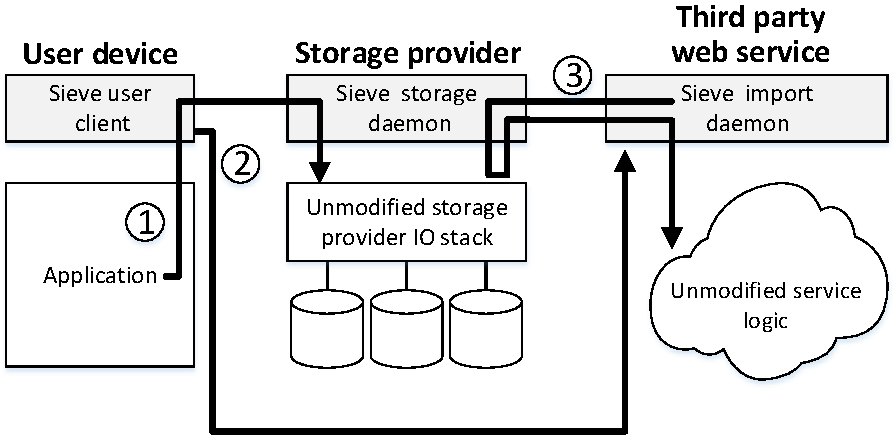
\includegraphics{figs/arch.pdf}
     \caption[Sieve's high-level architecture]
     {Sieve's high-level architecture. 1) The user uploads
              ABE-encrypted data to a storage provider. 2) The user
              generates a data policy for a third party web
              service. Sieve translates the policy into an ABE
              decryption key, and sends the key to the web service.
              3) The web service pulls encrypted data from the
              storage provider, decrypts it locally, and injects
              the data into the unmodified application pipeline.}
  \label{fig:sieve}
\end{figure}

\section{Our Solution}

To address these challenges, we propose Sieve,
a new system for delegating access to
private cloud data. Figure~\ref{fig:sieve} depicts
Sieve's high-level workflow. A user generates
raw data on her computational devices, and
uploads encrypted versions of it to a single cloud
repository; the user manages and pays for the 
cloud, not the web services which
desire access to the data. When a third party web service
requests access, e.g., during the first
time that a user visits a site, the user
generates a high-level access policy (\S\ref{sec:policies})
for the service. Sieve splits the policy into
two pieces: the storage provider learns which
objects a third party can access (but not the
cleartext versions of those objects), and the
third party learns the objects that it can
access, and the corresponding decryption keys,
while learning nothing about the rest of the
user's data set. Once the third party has
downloaded the necessary objects and decrypted
them, it feeds the cleartext data to a legacy
pipeline for processing user content (\S\ref{sec:attrGen}).

\begin{figure}
\centering
\begin{verbatim}
           (type="Fitness" OR type="Medical") AND (date > 2012) 
                          AND (source="FitBit") 
\end{verbatim}
\caption[Example Sieve policy]{Example Sieve policy for an exercise application.}
\label{fig:policyex}
\end{figure}

Sieve leverages three techniques to implement
the workflow in Figure~\ref{fig:sieve}:\\
\begin{smitemize}
  \item Sieve uses \textbf{attribute-based encryption}
  (ABE)~\cite{kpabe} to implement cryptographically strong access
  policies. In ABE, encrypted data is 
  associated with attributes, which are key-value 
  pairs like ``date=2012", and decryption keys are 
  associated with policies; a key can only
  decrypt whose attributes satisfy a key's
  policy. The policies and attributes are both
  stored in plaintext. Before the user uploads
  objects to the storage provider, she (or her local
  device) tags the objects with attributes like the
  date, the user's current location, or the object type
  (e.g., ``medical'', ``financial'', ``fitness").
  The uploading device transparently encrypts the objects
  with the relevant attributes before sending the objects to
  the storage provider. Later, when a third party web service 
  requests access to the user's data, the user creates a policy
  defined in terms of attributes and attribute
  operators like equality and less than. Figure~\ref{fig:policyex}
  shows an example of such a policy, which a user
  might give an application that visualizes her exercise data.
  The user's local device automatically translates the
  policy into an ABE decryption key, and sends the key
  to the web service. Afterwards, the web service can use
  the key to read the cleartext versions of the delegated
  objects from the storage provider and does not require
  any more communication with the user.
  
  \item To revoke a third party's access to sensitive data,
  the user informs the storage provider that the third
  party should no longer be able to download encrypted
  user objects. However, the third party still possesses
  the associated decryption key, and can decrypt leaked
  ciphertext if the storage server is later compromised.
  To prevent this scenario, Sieve uses \textbf{key
  homomorphism}~\cite{keyhom} to implement key revocation. Key
  homomorphism allows the storage provider
  to re-encrypt user data without learning the underlying
  cleartext--the storage provider merely reads the
  ciphertext and writes the output of a function that
  accepts the ciphertext and a user-specified rekeying
  token as input. The execution of this function on the storage 
  provider also does not reveal any information about the 
  cleartext data. Using \textit{in situ} re-encryption,
  users can avoid re-encrypting data on user devices and
  then re-uploading it. Additionally, if storage providers
  are honest at the time of key revocation, subsequent
  storage provider compromises will not reveal data that
  is encrypted with keys that are revoked (but possibly
  still in the wild). To our knowledge, Sieve is the first 
  ABE-based system to support full re-keying of \textit{both}
  the metadata and data.

  \item ABE uses a \emph{master secret key} to generate
  decryption keys. The loss of this key results
  in the compromise of the entire cryptosystem. In
  standard ABE schemes, the master secret is kept by a
  single trusted authority. In the context of Sieve,
  this would mean keeping the master secret on a single
  user device. This is unattractive, since user devices
  are often lost or stolen. Thus, Sieve
  uses \textbf{secret-sharing} and \textbf{two-factor
  authentication} to partition the master secret across
  multiple devices, and prevent unauthorized devices
  from arbitrarily participating in Sieve's cryptographic
  protocols.
    
\end{smitemize}

Sieve represents a middle ground between today's
popular web services (which provide weak user
control over the distribution and access of her data), 
and proposed systems from the
research community which strengthen user control,
but greatly restrict server-side computation~\cite{mylar}
or eliminate it altogether~\cite{sundr,depot,sporc,bstore,depSky}.
Sieve explores a
different point in the design space, one that
provides cryptographically strong access controls
to users while still permitting the rich
server-side computation on user's sensitive data
that many popular web
applications require to provide increased value
for the user.

To demonstrate its practicality, we integrated Sieve with
two different types of applications, a health application, 
Open mHealth~\cite{omh}, and a photo application, Piwigo~\cite{piwigo}.
Open mHealth is an open-source application that 
helps users store and visualize their data. We obtained
realistic user health data based on existing clinical standards
from Open mHealth and used Sieve 
to manage the user data (\S\ref{sec:integration}). Piwigo
is an open-source photo application that allows users to store
and manipulate their photos similar to Flickr~\cite{flickr}. 
Like Open mHealth, we used Sieve to manage the photos in Piwigo.
Integrating Sieve into the Open mHealth and Piwigo 
was straightforward and required approximately 200 and 250 lines of code
respectively. The experimental results show these integrated systems
can handle realistic workloads.